\begin{tikzpicture}
    \begin{scope}[x={(0mm,300mm)},y={(0mm,100mm)},line width=1pt,cap=round]
        \node[anchor=south west,inner sep=0mm] at (10mm,10mm) {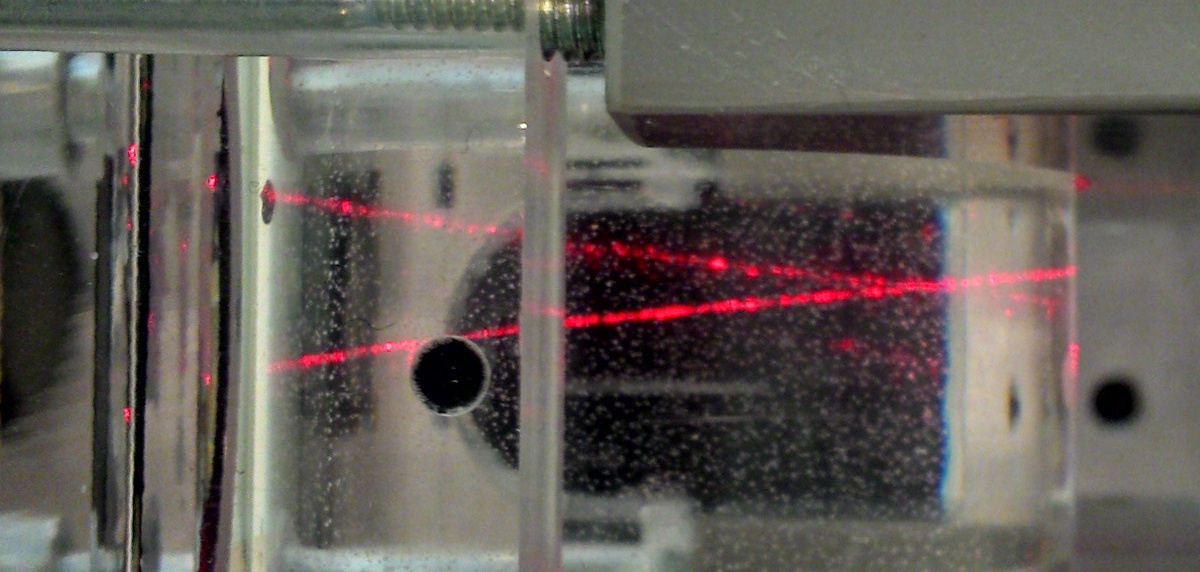
\includegraphics[width=260mm]{images/beams.jpeg}};

        \draw[-latex,line width=2pt] (5mm,30mm) -- (5mm,110mm);
        \node[rotate=90] at (1mm,65mm) {\huge{Wasserstr\"omung}};

        \draw[-latex,line width=2pt] (65mm,5.5mm) -- (230mm,5.5mm);
        \node at (150mm,0mm) {\huge{Einfallsrichtung Laserstrahlen}};
        %\draw[cyan] (210mm,80mm) -- (234mm,80mm);
        %\node[white] at (250mm,80mm) {\Large{\parbox{30mm}{\raggedright Geh\"ause mit \\Photomultiplier,\\ Blende und Linse $L_2$}}};
    \end{scope}
\end{tikzpicture}
